
\begin{figure}[H]
    \centering
    \begin{subfigure}[b]{0.3\textwidth} % default 0.25\textwidth
    %\begin{minipage}[t]{0.33\linewidth}
      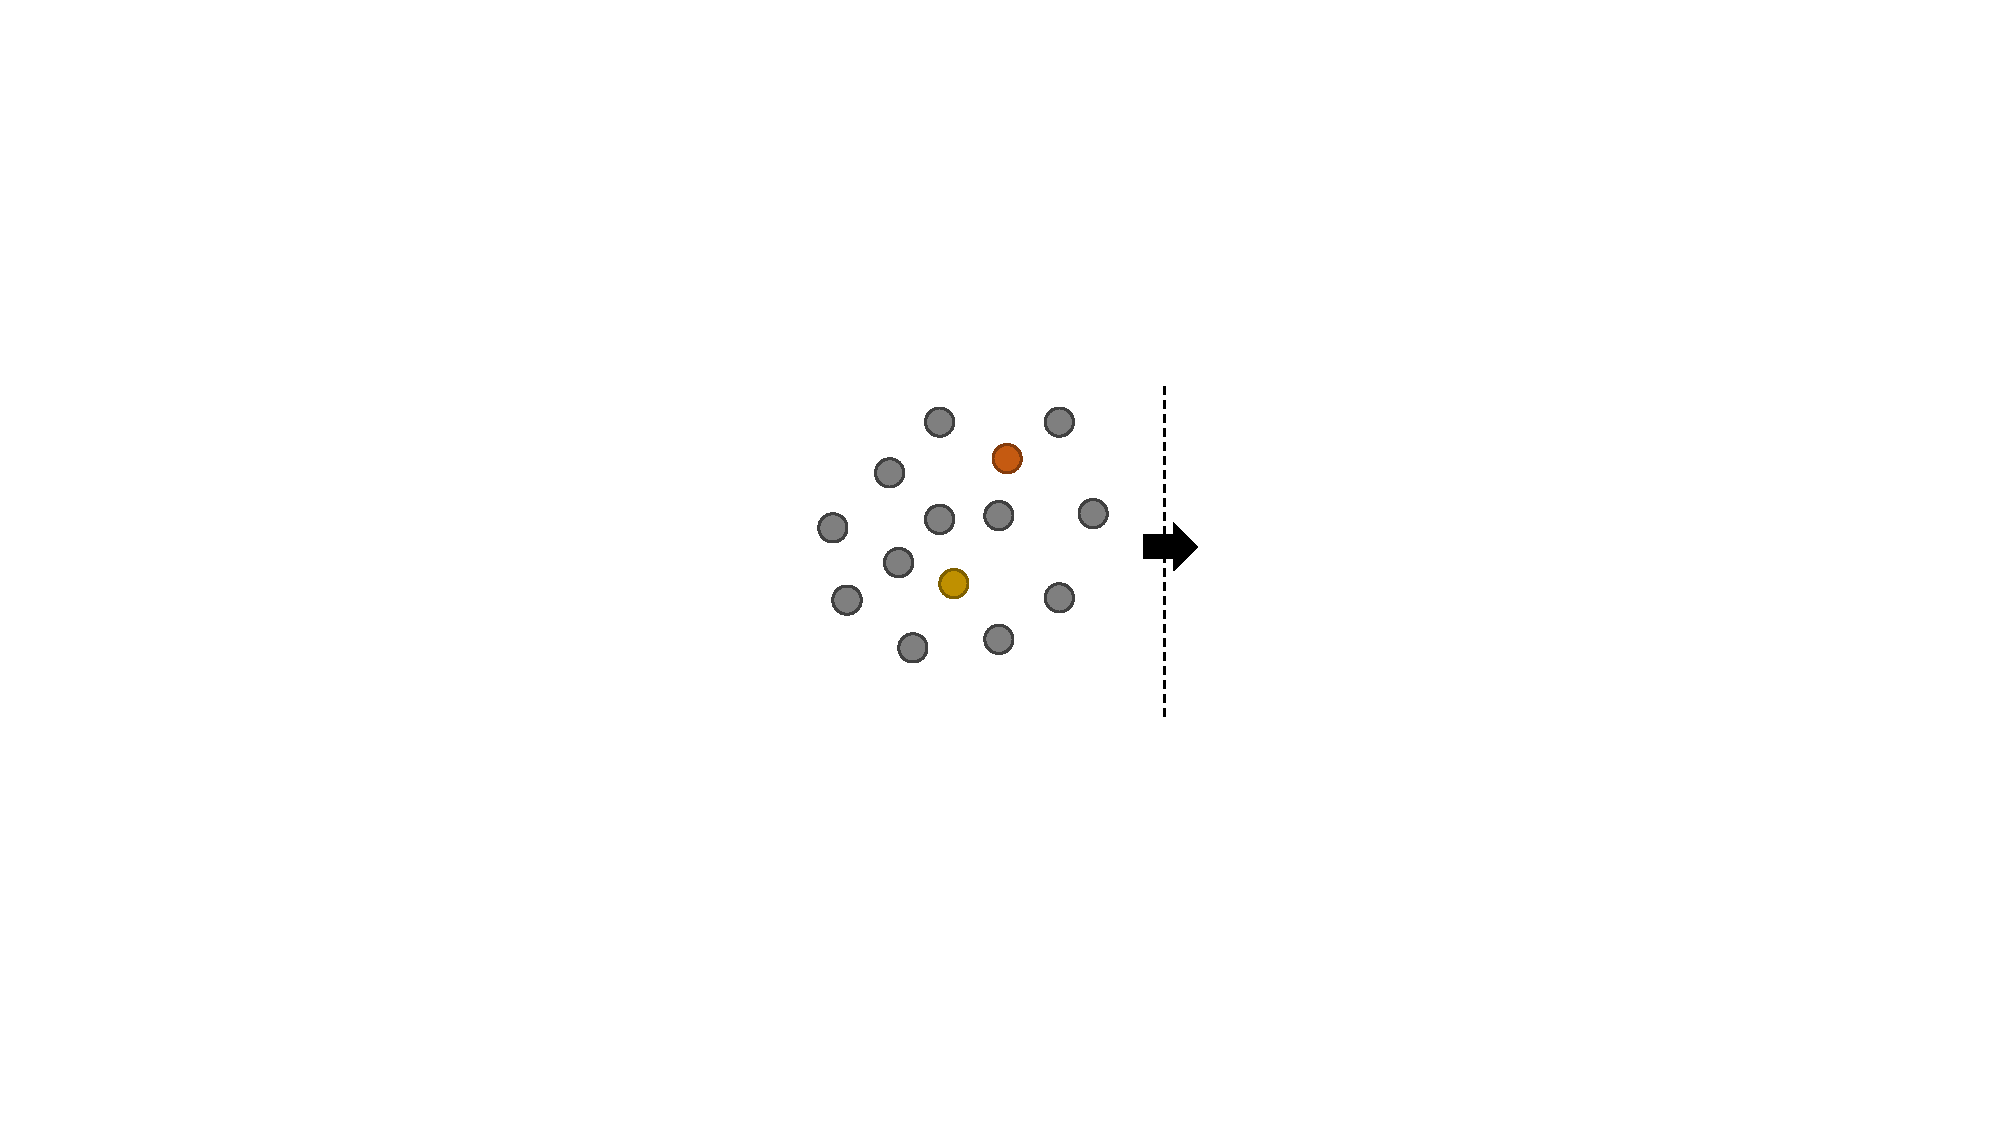
\includegraphics[width=\textwidth]{Img/fig_5_cat_a.pdf}
      \caption{}
      \label{fig:5_cat_a}
    %\end{minipage}
    \end{subfigure}%
    ~% add desired spacing
    \begin{subfigure}[b]{0.26\textwidth} % default 0.23\textwidth
    %\begin{minipage}[t]{0.33\linewidth}
      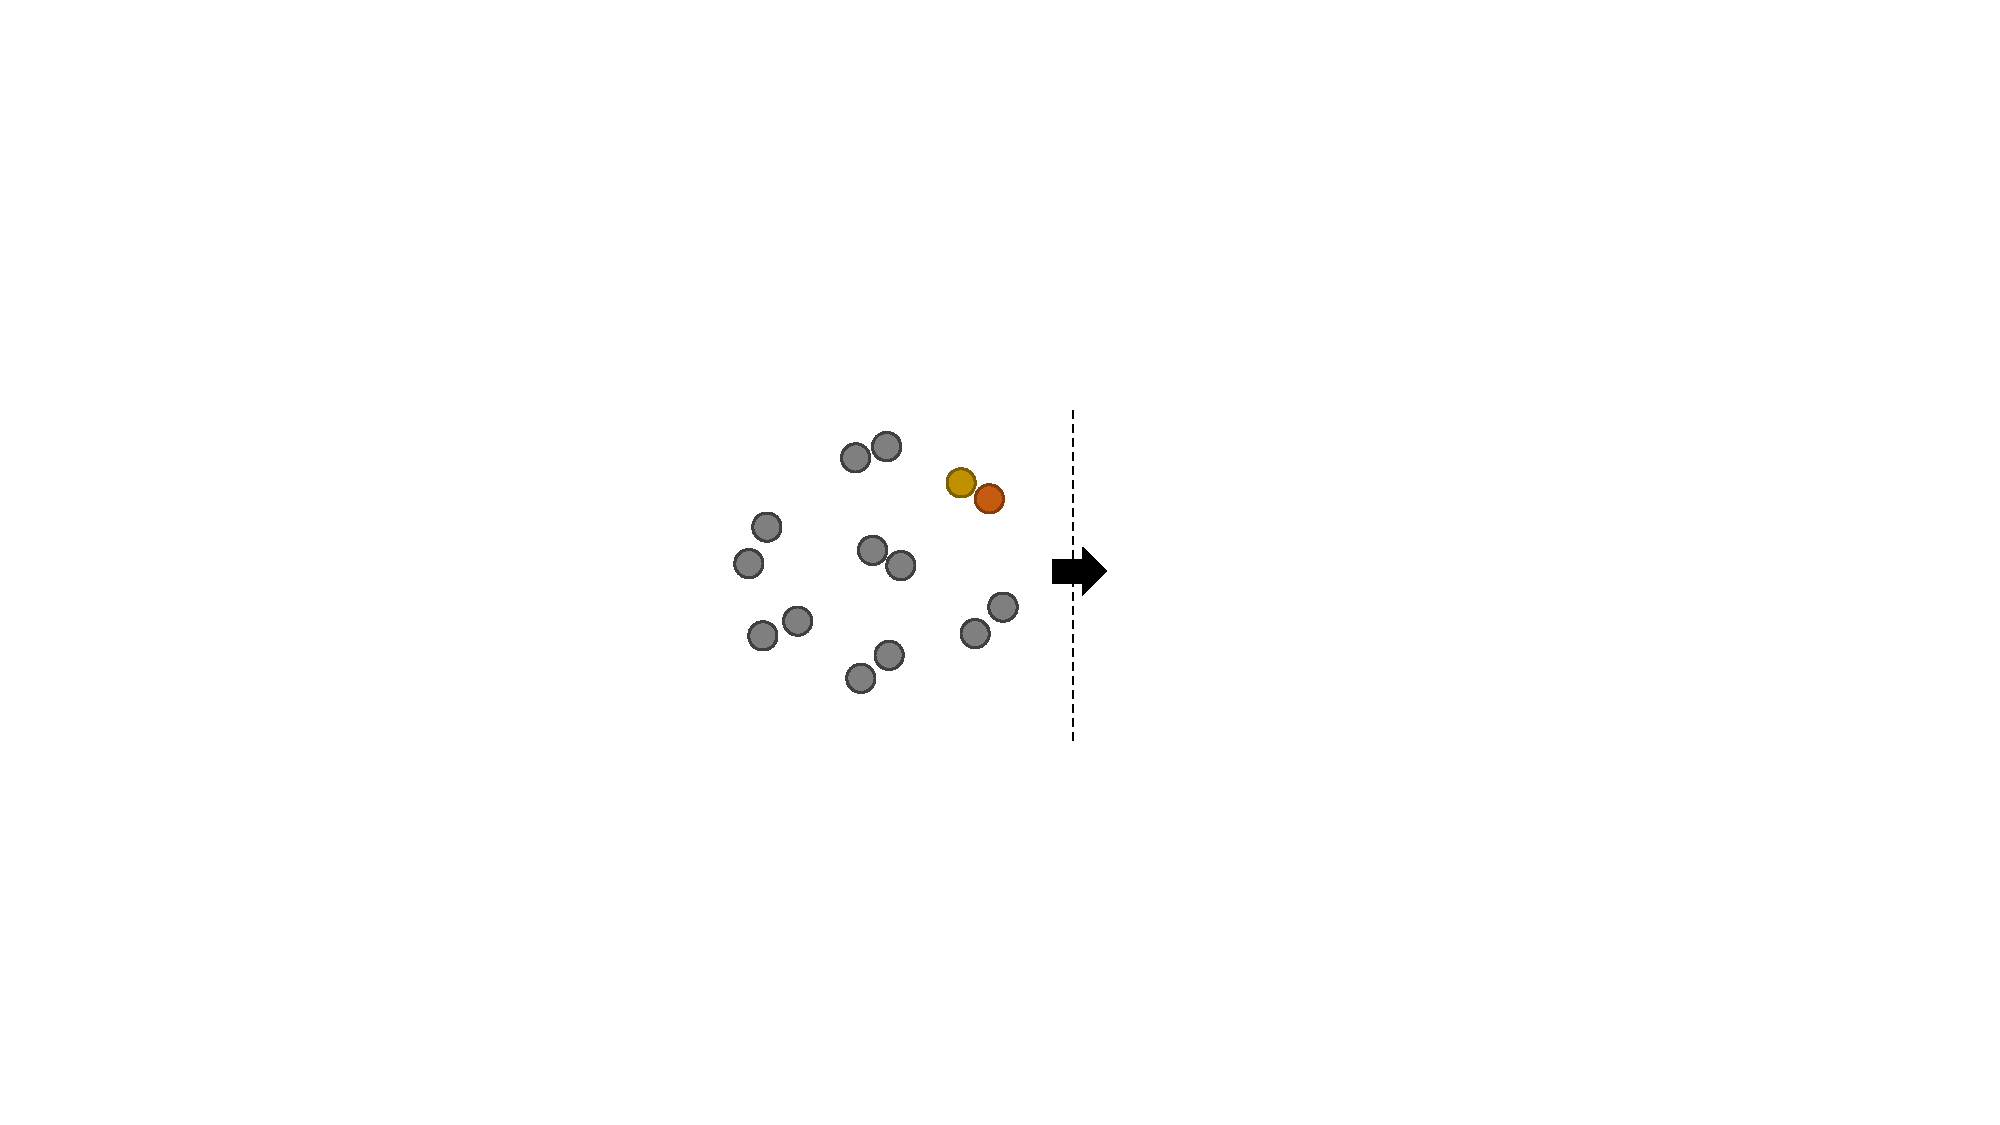
\includegraphics[width=\textwidth]{Img/fig_5_cat_b.pdf}
      \caption{}
      \label{fig:5_cat_b}
    %\end{minipage}
    \end{subfigure}
    % line break
    \begin{subfigure}[b]{0.38\textwidth} % default 0.32\textwidth
    %\begin{minipage}[t]{0.33\linewidth}
      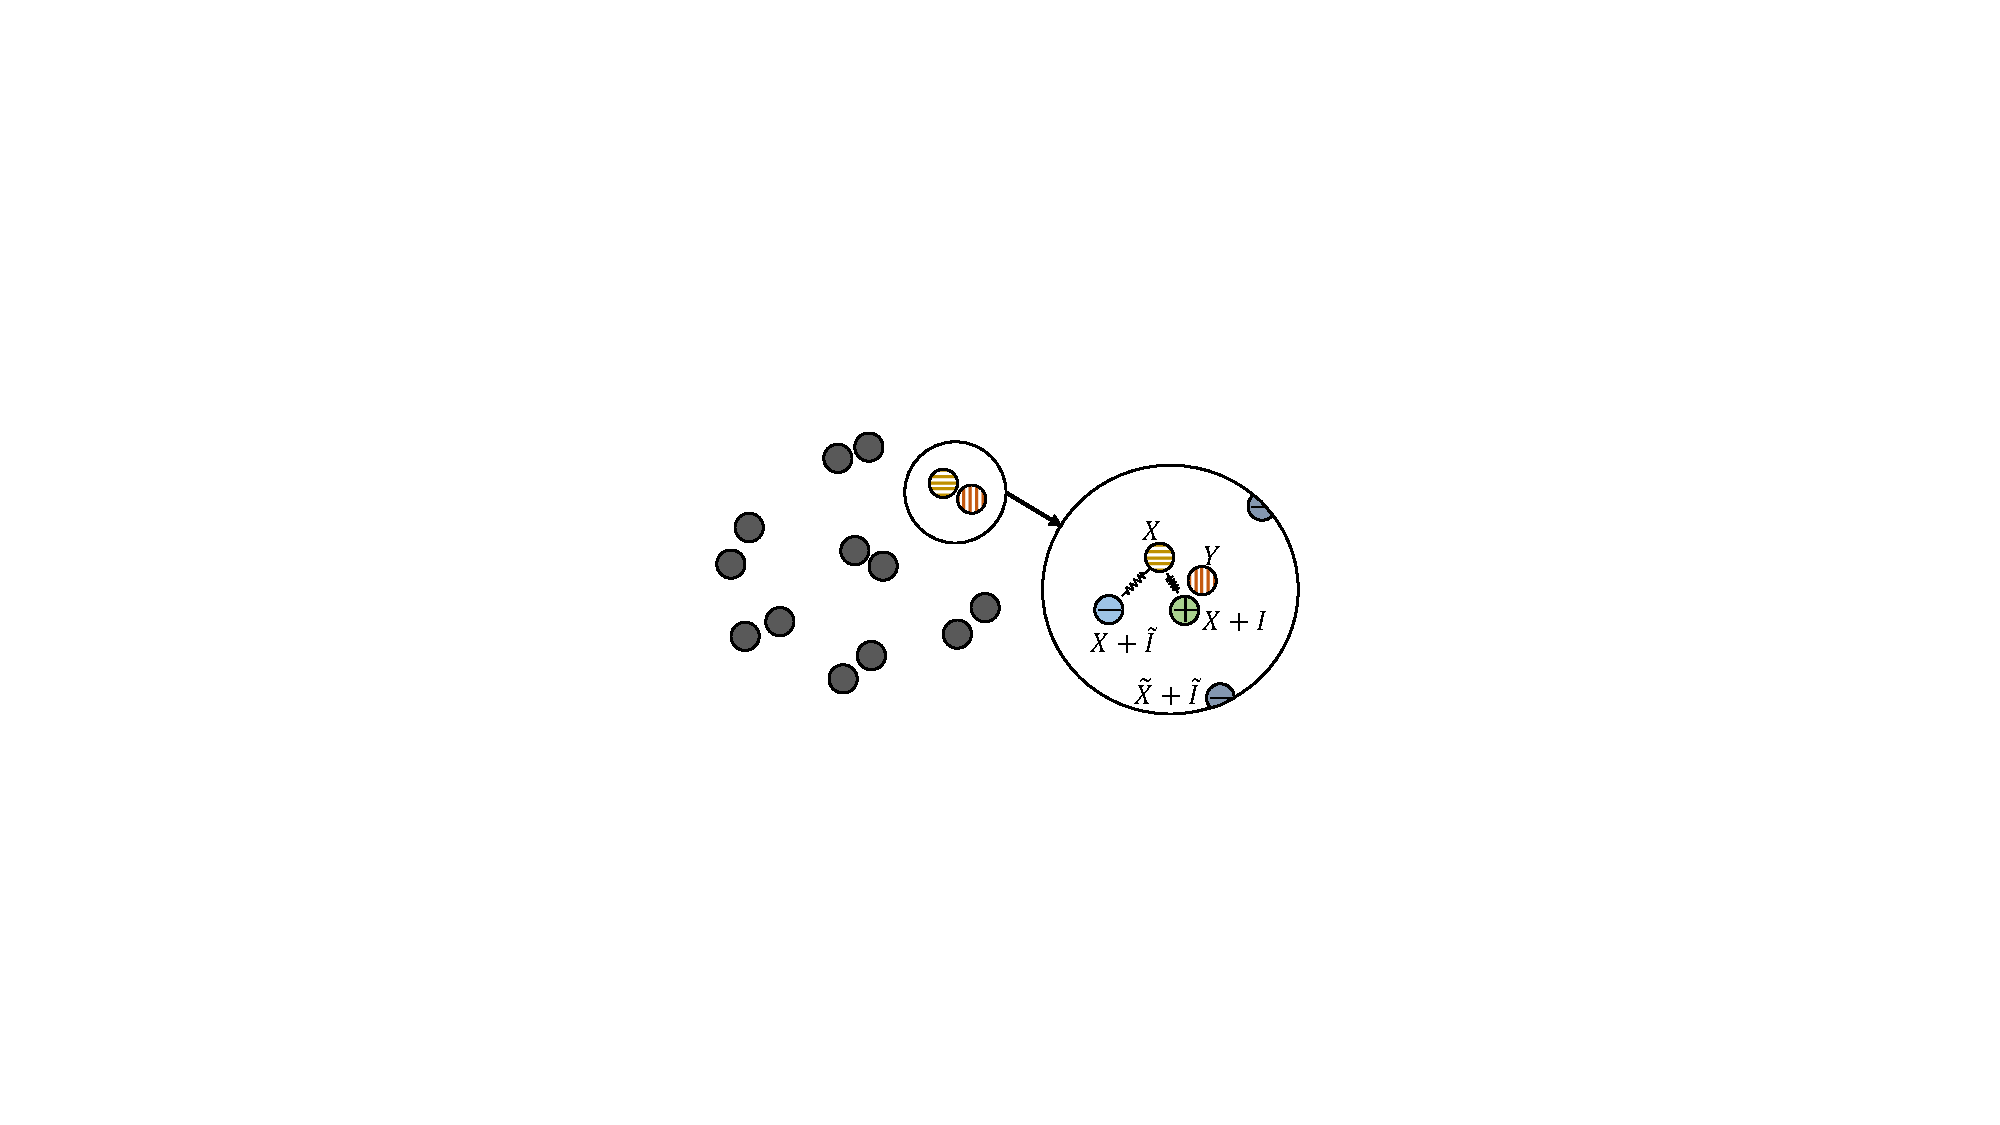
\includegraphics[width=\textwidth]{Img/fig_5_cat_c.pdf}
      \caption{}
      \label{fig:5_cat_c}
    %\end{minipage}
    \end{subfigure}%
    \bicaption{对比对抗训练方法原理示意图}{Schematic diagram of the principle of contrastive training method}
    \label{fig:5_cat}
\end{figure}